\documentclass[preprint,inputenc=ansinew,doublespace,notheorems,wider]{jeea}
%%%%%%%%%%%%%%%%%%%%%%%%%%%%%%%%%%%%%%%%%%%%%%%%%%%%%%%%%%%%%%%%%%%%%%%%%%%%%%%%%%%%%%%%%%%%%%%%%%%%%%%%%%%%%%%%%%%%%%%%%%%%%%%%%%%%%%%%%%%%%%%%%%%%%%%%%%%%%%%%%%%%%%%%%%%%%%%%%%%%%%%%%%%%%%%%%%%%%%%%%%%%%%%%%%%%%%%%%%%%%%%%%%%%%%%%%%%%%%%%%%%%%%%%%%%%
\usepackage{geometry}
\usepackage{pdfpages}
%\usepackage{graphicx}
%\usepackage{amsmath}
%\usepackage{amssymb}
\usepackage{float}
\usepackage{rotating}
%\usepackage[doublespacing]{setspace}
\usepackage[left]{eurosym}
\usepackage{dcolumn, array}
\usepackage{wasysym}
\usepackage{natbib}
%\usepackage[ansinew]{inputenc}
\usepackage{color}
\usepackage{subfigure}
\definecolor{dgreen}{cmyk}{1,0,1,0}
\usepackage[normalem]{ulem}         % \sout: strikeout; \uwave: waveline
%\usepackage{endfloat}

   \long\def\cmt#1{{\color{green}\sf\bfseries[#1]}}

% your comments and changes
    \long\def\ycmt#1{{\color{red}[{\slshape#1}]}}
    \long\def\yadd#1{{\color{red}\uwave{#1}}}
    \long\def\ydel#1{{\color{red}\sout{#1}}}

% Trax' comments and changes
    \long\def\tcmt#1{{\color{blue}[{\slshape#1}]}}
    \long\def\tadd#1{{\color{blue}\uwave{#1}}}
    \long\def\tdel#1{{\color{blue}\sout{#1}}}


\DeclareGraphicsExtensions{.jpg,.pdf,.mps,.png}

%\usepackage{endfloat} %Dieses package einschalten um die Tables und Figures ans Ende zu setzen!!
%\usepackage{endnotes}

\setcounter{MaxMatrixCols}{10}
%TCIDATA{OutputFilter=LATEX.DLL}
%TCIDATA{Version=5.00.0.2570}
%TCIDATA{<META NAME="SaveForMode" CONTENT="1">}
%TCIDATA{Created=Tue Oct 26 16:53:26 2004}
%TCIDATA{LastRevised=Tuesday, December 05, 2006 12:17:19}
%TCIDATA{<META NAME="GraphicsSave" CONTENT="32">}
%TCIDATA{<META NAME="DocumentShell" CONTENT="Journal Articles\Standard LaTeX Article">}
%TCIDATA{Language=American English}
%TCIDATA{CSTFile=LaTeX article (bright).cst}

%\newtheorem{result}{Result}
\textwidth=12.4cm \textheight=20cm
\setlength{\parskip}{1pt plus1pt minus1pt}
\oddsidemargin0.0cm \evensidemargin0.0cm \markright{}
\topmargin 1.0cm \topskip0.0cm \headsep0.8cm
\footnotesep0.3cm
%\interfootnotelinepenalty=10000
\clubpenalty=10000
\widowpenalty=10000
%\let\footnote=\endnote
%\input{tcilatex}

\setlength{\parskip}{1.0ex plus0.5ex minus0.5ex}
%\renewcommand{\baselinestretch}{2}

\begin{document}

\appendix

\begin{center}
\Large{\textbf{Online Appendix}}\\
\end{center}
\normalsize
\section{Text of cover letters}\label{sec:letters}
\renewcommand{\thefigure}{\Alph{section}.\arabic{figure}}
\renewcommand{\thetable}{\Alph{section}.\arabic{table}}
\renewcommand{\thefootnote}{\arabic{footnote}} \setcounter{footnote}{0}

\setcounter{figure}{0}
\setcounter{table}{0}
\setcounter{page}{1}




\subsection{Standard cover letter (baseline treatment T1)}
%\noindent{\textbf{1. Text of cover letters}} \smallskip

%\noindent \textbf{1.1 Standard cover letter (baseline treatment T1)}\smallskip

\footnotesize{
\noindent \textsl{Dear Mr. X,}\smallskip

\noindent \textsl{You listen to radio, you watch TV? Then you are aware of the program variety offered by Austrian Public Broadcasting. The provision of these services, however, requires funding. Therefore, everybody who owns a radio or a TV has to pay license fees. It is the task of} GIS Geb\"{u}hren Info Service GmbH \textsl{to ensure that all TV and radio consumers pay these fees.} \smallskip

\quad\quad\quad\quad\quad\quad\quad\quad\quad\quad\quad\quad\quad\quad\quad  [1]  \smallskip

\noindent \textsl{\textbf{Our database does not show a
registration of TV or radio equipment at your address.} This can
have several reasons:
\begin{itemize}
\item[--] We may have made a mistake in our database and you are
already registered at GIS. \textbf{In this case, we apologize in
advance.}
\item[--] Your registration data may have changed, e.g.,
due to a move or a name change (marriage), and our computer
system cannot match the data with your registration.
\item[--] You may not hold a radio or a TV at this address and therefore
do not have to register anything.
\item[--] Maybe you have just forgotten to register your TV or radio.
\end{itemize}
\noindent We are legally obliged to clarify this issue and kindly
ask you to answer our questions -- even if you have
already registered at GIS. On the back of this letter you will find a response form.
\textbf{Please fill in this form and send it back within the next 14 days.}} \smallskip

\quad\quad\quad\quad\quad\quad\quad\quad\quad\quad\quad\quad\quad\quad\quad  [2]  \smallskip

\noindent \textsl{We thank you for your cooperation. If you
require further information, please call our service hotline at
0810 00 10 80 (Monday to Friday, 8.00am to 9.00pm, Saturday from
9.00am to 5.00pm) or visit our web page at
www.orf-gis.at.}  \quad \quad \quad \quad \textsl{Kind regards, your} GIS--\textsl{Team.}
}\bigskip


%\normalsize{\noindent \textbf{1.2 Threat (treatments T2, T4, T6)}}\smallskip
\subsection{Threat (treatments T2, T4, T6)}
\small{\noindent Treatments T2, T4 and T6 included the following paragraph at position [2] of the standard letter:}

%\vspace{0.10cm}

\footnotesize{\noindent \textsl{\textbf{If you do not
respond to this letter, a staff member of GIS will contact you in
order to request information from you personally.} If you refuse
to provide information or if there is a well-founded suspicion that you provide disinformation, GIS is obligated to order an inquiry by the
responsible federal authorities. Please keep in mind that in this
case you may face legal consequences and considerable costs.}}

\newpage

\subsection{Social information (treatments T3, T4)}
%\normalsize{\noindent \textbf{1.3 Social information (treatments T3, T4)}}\smallskip

\small{\noindent Treatments T3 and T4 added the following paragraph at position [1] of the standard letter:}

\footnotesize{\noindent \textsl{\textbf{Do you actually know
that almost all citizens comply with this legal duty?} In fact, \textbf{94
percent} -- a vast majority of all households -- have registered
their broadcasting receivers.}}\medskip

\subsection{Moral appeal (treatments T5, T6)}
%\normalsize{\noindent \textbf{1.4 Moral appeal (treatments T5, T6)}}\smallskip

\small{\noindent The treatments T5 and T6 included the following paragraph at position [1]:}

\footnotesize{\noindent \textsl{\textbf{Those who do not
conscientiously register} their broadcasting receivers not only violate
the law, but also \textbf{harm all honest households. Hence,
registering is also a matter of fairness.}}}\bigskip

%\noindent \textbf{1.5 Original Copy} %\bigskip
%\begin{figure}[!h]
%\begin{center}
%\includegraphics[scale=0.70]{mailing.jpg}\\
%Original mailing for treatment T4 (Info $\times$ Threat)\\
%\QTR{caption}{Original mailing for treatment T4 (Info $\times$ Threat)}
%\end{figure}
%\end{center}
%\clearpage

\normalsize

\section{Evidence on the perceived level of non-compliance}\label{sec:perc_evasion}
%\noindent{\textbf{2. Survey on the perceived level of non-compliance}} \smallskip
\setcounter{figure}{0}
\setcounter{table}{0}

In a national survey conducted in the year 2000, more than 1000 Austrian households were asked to state their belief  about the frequency of license fee evasion \citep[see][]{traxler:09}. Figure \ref{belief} plots the distribution of the response (measured on a five-point Likert scale ranging from `very frequent' to `very infrequent') against GIS' estimate of the local evasion rate (in the categories 0-5, 5-10, 10-20, 20-30 and above 30\%) in the respondent's home district at the time of the survey. (The estimate for local evasion corresponds to one minus the share of households who are registered for license fees relative to the total number of households living in a jurisdiction.) The figure reveals a strong correlation of beliefs with the local evasion levels. In regions with an evasion rate below 5\%, more than 75\% believe that dodging the fee is infrequent or very infrequent. In districts with evasion levels above 30\%, this number drops to 33\%. Vice versa, the share of respondents who believe that evasion is frequent or very frequent rises from 11\% in low evasion regions to 34\% in districts with high levels of non-compliance. Estimating ordered probit models that control for individual characteristics confirms this correlation.

\begin{figure}[!h]
%\centering
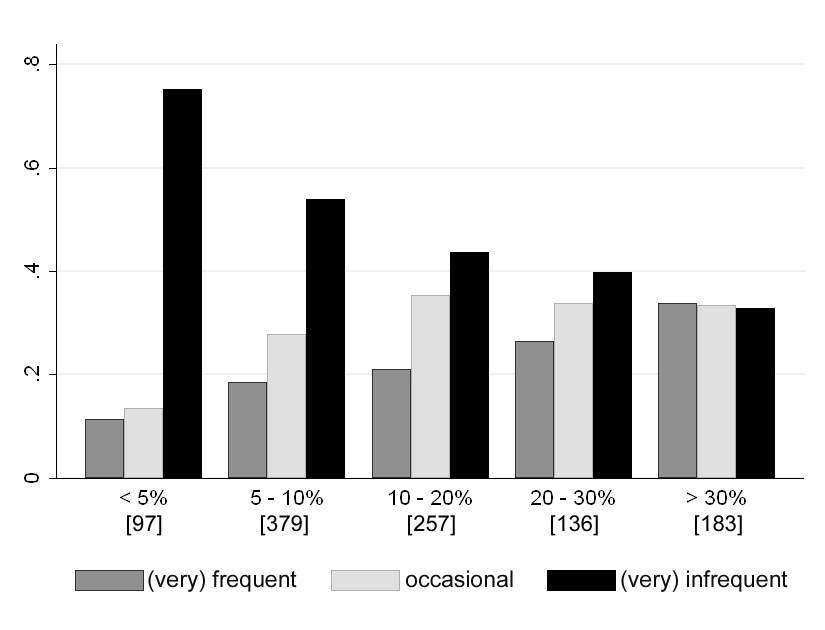
\includegraphics[width=12cm]{Belief2.jpg}
\caption{Beliefs about TV license fee evasion }\label{belief}
\centering \parbox{28pc}{\vspace{2mm}\footnotesize{\emph{Notes:} The figure plots the response distribution on beliefs about the frequency of license fee evasion in Austria for regions with an estimated local evasion rate of 0-5\%, 5-10\%, 10-20\%, 20-30\% and above 30\%. The number of observations in the five categories is displayed in squared brackets.}}
\end{figure}
\clearpage


\section{Heterogenous treatment effects}\label{sec:interactions}
%\noindent{\textbf{3. Interaction effects }} \smallskip

Table~C.1 presents the results from estimations of equation~(1) for several subgroups that split our sample according to the median of (i) the population size, (ii) population density, (iii) the municipalities' average household income, (iv) and the share of votes casted to rightist parties.\bigskip

\begin{table}[!h]
\caption{Heterogenous treatment effects}
\begin{center}\resizebox{16.0cm}{!}{
\begin{tabular}{lD..{4}D..{4}D..{4}D..{4}D..{4}D..{4}D..{4}D..{4}} \hline
        \hline
\multicolumn{9}{l}{Dependent variable: Registrations (within 50 days)} \\
\hline
      &	\multicolumn{2}{c}{Population Size}			&	 \multicolumn{2}{c}{Population Density}		 &	 \multicolumn{2}{c}{Household Income}			 &	 \multicolumn{2}{c}{Right Voters}			\\
 & \multicolumn{1}{c}{$\geq$median} & \multicolumn{1}{c}{$<$median} & \multicolumn{1}{c}{$\geq$median} & \multicolumn{1}{c}{$<$median} & \multicolumn{1}{c}{$\geq$median} & \multicolumn{1}{c}{$<$median} & \multicolumn{1}{c}{$\geq$median} & \multicolumn{1}{c}{$<$median} \\
\hline
 & \multicolumn{1}{c}{(I)} & \multicolumn{1}{c}{(II)} & \multicolumn{1}{c}{(III)} & \multicolumn{1}{c}{(IV)} & \multicolumn{1}{c}{(V)} & \multicolumn{1}{c}{(VI)} & \multicolumn{1}{c}{(VII)} & \multicolumn{1}{c}{(VIII)} \\
\hline
Threat & 0.017^{***} & 0.008^{**} & 0.014^{***} & 0.011^{***} & 0.020^{***} & 0.006^{**} & 0.006^{*} & 0.018^{***} \\
 & (0.004) & (0.004) & (0.004) & (0.004) & (0.005) & (0.003) & (0.003) & (0.004) \\
Moral & -0.002 & -0.008^{*} & -0.001 & -0.010^{**} & -0.004 & -0.005 & -0.007^{*} & -0.003 \\
 & (0.005) & (0.004) & (0.005) & (0.004) & (0.005) & (0.004) & (0.004) & (0.005) \\
Info & -0.002 & -0.002 & 0.000 & -0.005 & -0.000 & -0.004 & -0.002 & -0.003 \\
 & (0.005) & (0.004) & (0.005) & (0.004) & (0.005) & (0.004) & (0.004) & (0.005) \\
 \hline
Observations & \multicolumn{1}{c}{20,528} & \multicolumn{1}{c}{20,479} & \multicolumn{1}{c}{20,726} & \multicolumn{1}{c}{20,281} & \multicolumn{1}{c}{18,438} & \multicolumn{1}{c}{22,569} & \multicolumn{1}{c}{20,521} & \multicolumn{1}{c}{20,486} \\ \hline \hline
\end{tabular}}\\[2ex]
\tablenotes*{\footnotesize{ \emph{Notes:} All specifications are estimated with a linear probability model and include a constant term and a large set of control variables \citep[see][]{fellner:09}. The estimations are run for subgroups that split the sample according to the sample median of the municipalities population size (I and II), population density (III and IV), average household income (V and VI) and the share of votes casted to rightist parties (\emph{Volkspartei}, \emph{Freiheitliche} and \emph{B\"{u}ndnis Zukunft \"{O}sterreich}) in the 2006 parliamentary elections (VII and VIII). Robust standard errors are in parentheses. $^{\star\star\star}$, $^{\star\star}$, $^{\star}$ indicate significance at a 1\%, 5\%, 10\%-level, respectively.}}
\end{center}
\end{table}
\bigskip

\section{Perception survey}\label{sec:survey}
%\noindent{\textbf{4. Perception survey}} \smallskip
\setcounter{figure}{0}
\setcounter{table}{0}
\subsection{Details on setup and procedure}
%\begin{center}
%\large{\textbf{Appendix~V: Details on the Manipulation Check}}\\
%\end{center}
%\section*{Appendix~V: Details on the Manipulation Check}
The perception survey was implemented November 24--28, 2008, using the online survey tool \emph{unipark.de}. Survey participants were invited via email on the University of Innsbruck mailing list. To provide an incentive for participating, everybody who finished the survey had a 1/25 chance of winning an Amazon voucher worth \euro \thinspace25.  4,165 individuals clicked on the link to the survey and 3,233 completed the survey within an average of 8 minutes. The participants were mainly students plus some non-academic employees. Hence, the subject pool differs substantially from the sample of our field experiment. However, there should be a relatively high fraction of evaders in the survey sample, as cheating on license fees is quite common among students.

Survey participants were randomly confronted with one of two scenarios. One scenario described an evader vignette (a person who moved to a new place six months ago  and evaded the fee since then), the other one a vignette of a complying individual (who moved six month ago, paid the fee, but did not inform GIS about the change in address). After participants read the scenario description, the web page randomly linked them to a situation that mimicked one of the treatments from the field experiment. A random subsample formed the control (T0). All others were instructed that the vignette person received a mailing from GIS. Thereafter a cover letter, which corresponds to one of our six mailing treatments (T1--T6), was displayed on the web page. Survey participants were then asked to evaluate the situation of the person. In this way, we elicited the treatments' impact on various perceptions.

The question regarding the perceived risk of an inspection was formulated as follows: \normalsize{``\textit{How large do you think is the risk -- after having received this mailing} [omitted for the control group (T0)] \textit{-- that the person will receive a `visit' by a licensing inspector within the next 4 weeks? Please tick a number on the scale between 0 (very unlikely) to 100 (very likely).}''} Note that subjects had to click on a very fine-scaled ruler to indicate this number. Hence, our data show comparably little clustering on prominent numbers.\smallskip \\
%
\normalsize{A question regarding the perceived inclination to respond to the treatment -- either by registering (for evaders) or by making an update response (for complying individuals) -- was asked in a similar way:} \normalsize{``\textit{What do you think is the person's inclination -- after having received this mailing} [omitted for the control group (T0)] \textit{-- to register at GIS within the next 4 weeks and pay the license fee thereafter?} [\textit{... to inform GIS about the new address within the next 4 weeks?}] \textit{Please tick a number on the scale between 0 (will certainly not register [inform]) to 100 (will certainly register [inform]).}''}\smallskip \\
%
\normalsize{We also asked for the expected fines in case of a detection: ``\textit{Assume that the person is indeed detected by a field inspector. Which  consequences do you expect? He has to pay...}\\
 \small{ (1) \textit{no fine}.\\
 (2) \textit{a fine of less than \euro 100}.\\
 (3) \textit{a fine of \euro 100 -- 500}.\\
 (4) \textit{a fine of \euro 500 -- 1000}.\\
 (5) \textit{a fine of \euro 1000 -- 2000}.\\
 (6) \textit{a fine of \euro 2000 -- 4000}.\\
 (7) \textit{a fine of more than \euro 4000}.''}\smallskip \\

\clearpage
\noindent \normalsize{Expectations regarding social sanctions were elicited in the following way:} \\
\small{``\textit{An acquaintance of the person learns that he has not paid TV license fees for the past 6 months.} [\textit{...that he has not informed GIS about his change in the address.}] \textit{How will the acquaintance react?}\\
 (1) \textit{will strongly approve the behavior, and support him not to register for license fees} [\textit{not to update the information}].\\
 (2) \textit{will approve the behavior}.\\
 (3) \textit{will not react at all}.\\
 (4) \textit{will disapprove the behavior}.\\
 (5) \textit{will strongly disapprove the behavior, and cool down the contact to the person}.}

\subsection{Survey results}

\normalsize{Columns (I) and (II) of Table \ref{tab:survey:risk} show the outcome of regressing the stated risk perception on the treatments and the scenario type. By far the largest impact on perceptions is induced by the mailing conditions. After being confronted with a mailing, survey participants evaluate the household's inspection risk to be roughly 60\% higher than in the no-mailing group.\footnote{The percentage is based on the estimates from specification (I) in Table~\ref{tab:survey:risk}, putting the coefficient for the mailing dummy relative to the constant.} Compared to the baseline mailing (T1), the threat increases the expected inspection risk by another 5\%. Specification (II) includes control variables on the respondents' personal characteristics. This hardly changes the point estimates of the treatment effects. The same holds true when we estimate Tobit instead of OLS regressions. Remarkably, similar estimations for perceived \emph{social} sanctions reveal that the threat -- just like the two other mailing conditions -- does not affect respondents' expectations.} %This result corroborates the view that the threat does not evoke a social dimension.

\begin{table}[!h]
\caption{Survey results: Treatment effects on risk perceptions and propensity to respond}\label{tab:survey:risk}
\begin{center}\resizebox{12.0cm}{!}{
 \begin{tabular}{lD..{4}D..{4}D..{4}D..{4}} \hline \hline
\multicolumn{1}{l}{Dependent variable:} & \multicolumn{2}{c}{Inspection risk} & \multicolumn{2}{c}{Response propensity}  \\ \hline
& \multicolumn{1}{c}{(I)} & \multicolumn{1}{c}{(II)} & \multicolumn{1}{c}{(III)} & \multicolumn{1}{c}{(IV)}\\ \hline
Mailing & 22.923^{\star\star\star} & 24.333^{\star\star\star} & 39.490^{\star\star\star} &  40.699^{\star\star\star}  \\
\vspace{4pt} & (2.179) & (2.183) & (1.697) & (1.713) \\
Mailing $\times$ Threat& 2.921^{\star\star\star} & 3.193^{\star\star\star} & 5.132^{\star\star\star} & 5.621^{\star\star\star}\\
\vspace{4pt} & (1.104) & (1.107) & (0.957) & (0.944)\\
Mailing $\times$ Moral & 0.768 & -0.056 & 1.667 & 0.702 \\
\vspace{4pt} & (1.332) & (1.338) & (1.152) & (1.141) \\
Mailing $\times$ Info & -0.306 & -1.064  & 3.083^{\star\star} & 2.597^{\star\star} \\
\vspace{4pt} & (1.360) & (1.362) &  (1.180) & (1.156) \\
Evader & 0.673 & 0.862 & -7.063^{\star\star\star} & -7.095^{\star\star\star}\\
\vspace{4pt} & (1.103) & (1.104) & (0.954) & (0.941)\\
Constant & 38.388^{\star\star\star} & 56.801^{\star\star\star} & 26.448^{\star\star\star} & 59.561^{\star\star\star} \\
 & (2.106) & (5.354) & (1.614) & (4.379) \\ \hline
%\vspace{4pt} &  &  \\
%GIS28
% $R^2$ & 0.049 & 0.086 \\ \hline
Additional control & \multicolumn{1}{c}{No} & \multicolumn{1}{c}{Yes} & \multicolumn{1}{c}{No} & \multicolumn{1}{c}{Yes} \\ \hline
Observations & \multicolumn{1}{c}{3,213} & \multicolumn{1}{c}{3,098} & \multicolumn{1}{c}{3,213} & \multicolumn{1}{c}{3,098} \\ \hline \hline
\end{tabular}}\\[1ex]
\tablenotes*{\footnotesize{ \emph{Notes:} Results from OLS regressions with robust standard errors in parentheses. $^{\star\star\star}$, $^{\star\star}$ indicate significance at a 1\%- and 5\%-level, respectively.}}
\end{center}
\end{table}

\normalsize{Columns (III) and (IV) of Table \ref{tab:survey:risk} report the estimated treatment effects on the expectations about the vignette person's propensity to respond to the treatment (either by registering or by updating). In line with the treatment effects on the perceived risk of an inspection, and consistent with the results from the field experiment, survey participants expect a strong mailing effect and a modest, but significant additional effect of the threat. In addition, the survey data also indicate a positive effect of the social information treatment. This observation might be explained by the fact that the survey participants initially expected a relatively low level of compliance (with a mean of 70.5\% and modus of 75\%) and were therefore positively surprised by the information on a compliance rate of 94\%. Finally, the regressions also show that evaders are expected to be less likely to respond compared to complying individuals. Again, this mirrors the gap in the frequency of registrations and update responses observed in the field experiment.}

\normalsize{Regarding the expected size of fines, we find neither an impact of the threat nor any mailing effect. The survey reveals, however, that participants expect significantly lower fines for complying individuals than for cheaters ($p=0.003$, according to a Wilcoxon rank-sum test). Equivalently, complying households are also expected to face significantly weaker social sanctions in case of an inspection ($p=0.003$). These findings are consistent with the fact that GIS does not impose fines on law-abiding individuals and supports our interpretation of the heterogenous impact of the threat on registrations and update responses established in the field experiment (see Section~5.2).

\renewcommand{\bibname}{References}
\renewcommand{\baselinestretch}{1.5}
\bibliography{compliance}

\bibliographystyle{jeea} \clearpage

\end{document}